
%(BEGIN_QUESTION)
% Copyright 2009, Tony R. Kuphaldt, released under the Creative Commons Attribution License (v 1.0)
% This means you may do almost anything with this work of mine, so long as you give me proper credit

Suppose we needed to connect a variable resistor in series with a sensitive analog meter movement to range that meter for a certain maximum voltage, and we were going to make all connections using a terminal strip.  Draw connecting wires that will create a {\it series} circuit between the meter and two terminals of the potentiometer, such that polarity of the applied voltage will be correct for the meter with the red test lead being positive and the black test lead being negative:

$$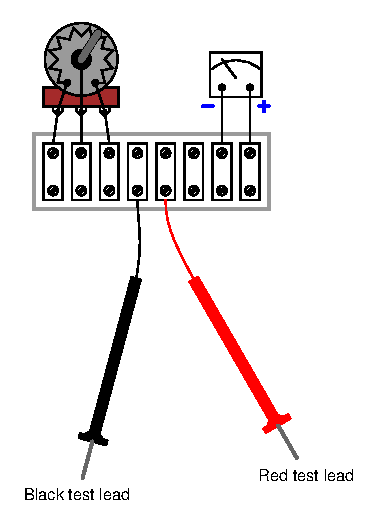
\includegraphics[width=15.5cm]{i03809x01.eps}$$

\underbar{file i03809}
%(END_QUESTION)





%(BEGIN_ANSWER)

Bear in mind that this is not the {\it only} possible circuit solution:

$$\includegraphics[width=15.5cm]{i03809x02.eps}$$

Challenge yourself by designing a different circuit to meet the same criteria! 

%(END_ANSWER)





%(BEGIN_NOTES)

%INDEX% Pictorial circuit review (analog voltmeter circuit)

%(END_NOTES)


